\documentclass[conference]{IEEEtran}
\IEEEoverridecommandlockouts
\usepackage{cite}
\usepackage{amsmath,amssymb,amsfonts}
\usepackage{algorithmic}
\usepackage{graphicx}
\usepackage{textcomp}
\usepackage{xcolor}
\usepackage{booktabs}
\usepackage{color,soul}
\def\BibTeX{{\rm B\kern-.05em{\sc i\kern-.025em b}\kern-.08em
    T\kern-.1667em\lower.7ex\hbox{E}\kern-.125emX}}
\begin{document}

\title{Regime Alpha: A Novel Universal Benchmarking Framework for Regime-Conditional Strategy Evaluation}

\author{\IEEEauthorblockN{Sagar Tanwar}
\IEEEauthorblockA{\textit{School of Computer Science and Engineering} \\
\textit{Galgotias University}\\
Greater Noida, India \\
33.sagartanwar@gmail.com}
\and
\IEEEauthorblockN{Nidhi Agarwal}
\IEEEauthorblockA{\textit{School of Computer Science and Engineering} \\
\textit{Galgotias University}\\
Greater Noida, India \\
nidhiagarwal82@gmail.com}
}

\maketitle

\begin{abstract}
Financial markets are non-stationary, and despite the fact most algorithmic strategies assume static conditions which essentially translates to expecting the future would be exactly similar as the past and, hence mirroring it. We already have regime-aware models like HMMs and changepoint detectors in existence but lack a standardized framework which can be used to test arbitrary strategies against these market shifts. We propose ``Regime Alpha'', it is a universal benchmarking platform,\hl {which in this context refers to architectural generality of this framework instead of exhaustive empirical coverage, the system} leverages the Decorator pattern to wrap any trading strategy with an unsupervised HMM layer. To validate and test this system, we conducted a 25-year empirical analysis on SPY ETF. We compared a standard mean reversion strategy against itself but with regime aware properties and it exhibited a dramatic reduction in the risk and maximum drawdown with respect to its raw format, especially during 2008 and 2020 financial crises. This confirms that regime alpha operates independently of strategy logic and shows its capabilities as a testing and evaluation tool for developers and strategists to test their strategies with regime aware features.
\end{abstract}

\begin{IEEEkeywords}
Algorithmic Trading, Financial Market Regimes, Hidden Markov Models, Non-Stationary Time Series, Strategy Benchmarking, Risk Management, Regime-Aware Models, Quantitative Finance
\end{IEEEkeywords}

\section{Introduction}

Financial markets are not stationary in nature, means their statistical properties like mean, variance and correlation keep changing over time, this phenomenon essentially is the result of countless variables which affect any financial asset that is being publicly traded like, the Political Events, Geopolitical moves, public sentiments, macroeconomic changes like the ones experienced during the 2008 Global Financial Crisis or the 2020 Covid Pandemic. They create moments that we also call ``Structural Breaks'', result in periods of extreme volatility and get unpredictable for traditional models to predict, especially using standard technical parameters only. In order to get above this issue, the idea of regime detection as a separate layer is implemented which acts as a filter to the trade execution process. Currently most trading systems are often trained on the historical market data while under the assumption that markets would act exactly the same as they did in the data. The result for this process becomes that the models perform very brilliantly in the back testing situations and catastrophically failing when the market conditions change to volatile giving these strategies noise which they interpret as signals at which point the profits and losses are no longer mathematically strategized results but numbers depending on random chance and needless to say is undesirable in such domain as it can result in massive drawdowns and capital degradation. This work's contribution is architectural and methodological providing a regime-conditional evaluation framework rather than a standalone Strategy. 

While the existing literature is filled with countless regime-specific, regime-aware, regime-switching models. There is still a notable absence of a generalized open-source framework that allows for universal benchmarking of the trading strategies and effectiveness with and without regime detection. Current practitioners who make trading strategies are required to hardcode the regime framework in the trading logic, which sometimes can be tacky to deal with and result in some issues related to the manipulation of actual trading logic. The manual process hence is wildly inefficient and also doesn't provide an insight into the fact if we even need regime detection for our system as there is a possibility that the system already is robust enough that it's able to survive the noise, in that scenario the regime systems would just be adding additional filters reducing the number of opportunities which would have been potentially profitable. Now to simply plug in our strategy and evaluate its performance relative to the same strategy but with a regime filter, it'd help to evaluate the strategy and get an insight into its capabilities if it was paired with a regime detector.

To come up with a solution we have ``Regime Alpha'', a Modular Open-source benchmarking framework that works independently of Strategy logic and Market state (Regime detection), i.e. what to trade and how to trade. In order to achieve this capability, this project utilized a multi-disciplinary approach combining software engineering with probabilistic modelling. To be specific this model is built upon the Decorator Design Pattern, it is a structural pattern that allows the specific behaviour to be added to individual objects, dynamically and at the same time now affecting the behaviour of the other objects from the same class, This is paired with the Gaussian Hidden Markov Model(HMM), which acts as the inference engine for detecting the latent regimes/ market states(Bull market, Bear Market, Ranging, Choppy, etc.). By using these domains, this system creates a decoupled architecture where the strategy logic is unchanged which the regime detection logic works like a safety guard which prevents the strategy to trade during the moments with high unpredictability which are the moments where it's most likely that the model will simply collapse by not being able to properly interpret the signals. This research is focused on the implementation and evaluation of the effectiveness of the framework, getting insights about how this could help in evaluating strategies such that their capabilities with and without regime-detection systems are apparent.

The analysis uses the S\&P 500 ETF(SPY) as the primary dataset for market data covering a 25 Year daily OHLC data and uses a basic mean reversion strategy which is very much underperforming so much so it burnt most of the capital by 2008 only. Plugging the said strategy prevents it from staying live in the moments where the regime is highly volatile. It's crucial to mention that while the framework supports multiple ML models for regime detection, this paper still focuses mainly on the Gaussian HMMs due to their interpretability and established presence in financial literature. Furthermore, the study prioritizes the primary goal of minimizing the risk and let the strategy worry about squeezing the profits out of the market. This project has a huge scope where we can further introduce the models where instead of just preventing the user provided strategy to trade in the volatile regimes, a possibility to multi-dimensional analysis and invert the strategy logic or manipulate it such that with minimizing risk it also potentially increases profitability. Which can further provide an interactive and quick insight on different risk aversion models and strategies which users can implement in their code as per the requirements.

\section{Literature Review}

One of the earlier claims facilitating the fact of non-stationarity of market was provided in \cite{b1}, which explored that the GNP growth is better modelled as a 2 state regime process, recession and growth states instead of what autoregressive models suggest, and these switching of states are autocorrelated, so if the economy shifts towards a certain state, it tends to stay in that state for a while before switching. Markov-Regime switching Models to capture these business cycles were proposed in \cite{b1}. The intuitive approach of HMMs and their practical implementation were explained in \cite{b2}, and the Hidden Markov Model's working and effectiveness in real speech recognition tasks were also demonstrated. This gave an insight that this could be expanded as HMMs treat regimes as probabilistic hidden states rather than deterministic labels. Building on this, regime-switching models were implemented for international asset allocation in \cite{b3}, showing that expected returns, volatilities and cross-asset correlations are dependent on regimes. It was shown that the regime-based portfolio outperformed the static strategies in terms of risk-adjusted returns. The Adaptive Markets Hypothesis (AMH) was proposed in \cite{b4}, as a complementary perspective on the previous work, which described the market efficiency as an evolving property that is driven by investor learning, competition and adaption. This work explicitly explained that optimality of static notions is straight up wrong. AMH despite being a great justification of adaptive and regime aware trading systems, it still was just more of a philosophical rather than an operational model.

An empirical comparison of regime-based and static asset allocation strategies was conducted in \cite{b5}, where HMMs were applied to detect hidden market states directly from return data. The results from this comparison proved that allocation rules conditioned on detected regimes improves the downside risk and risk-adjusted performance. Likewise, it was shown in \cite{b6} that Markov regime-switching models can enhance Portfolio selection by allowing returns to be modelled differently depending on the hidden market state. The descriptive relevance of these models was further strengthened in \cite{b7}, as regime-dependent return and volatility dynamics in markets were identified. However, their analysis was more focused on improved statistical fitting and inference accuracy rather than profitability. One of the initial formal definitions of concept drift was provided in \cite{b8}, showing that models can degrade in scenarios where data distribution changes overtime. This work focused on adaptation by retraining and weighting recent data, however this didn't use any latent regime structures or had any relevance with financial strategies.

A survey of concept drift detection and adaptation methods in machine learning was presented in \cite{b9}. Different types of drifts such as abrupt, gradual, and recurring were defined. These can be mapped to financial regimes, cycles and structural changes. The focus for this work was on predictive accuracy and ML metrics, not related to economic domain or trading performance. Computational methods in financial markets with emphasis on non-stationarity and drift were surveyed in \cite{b10}, showing that many financial ML systems already assume changing data and adapt reactively, but that adaptivity was handled by retraining or updating models with no explicit hidden regime layer or a strategy evaluation framework. An architecture for drift handling with a clear separation between detection, representation and response was proposed in \cite{b11}. This still was focused on predictive tasks and ML based performance rather than financial returns. The use of HMMs for robust regime detection and changepoint identification in equity and volatility markets was discussed in \cite{b12}. It was shown that instead of forcing long memory into the model with a mathematical constraint, long memory can emerge naturally from realistic market behaviour (stable regimes that slowly evolve). This made these regime-switching models structural and forecast-effective.

Explainable features based on HMM that identify both latent market regimes and the features driving each regime were introduced in \cite{b13}, providing improved transparency and interpretability. It was shown in \cite{b14} that ML models can benefit when the data generating process is modelled as regime dependent, where regime effects are absorbed into the prediction model itself rather than treated as a separate signal. However, there was no independent regime module or strategy level framework in this work. Regime switching was used as a part of adaptive exit dynamics in \cite{b15}, where the edge was based on a trend following system, making regime awareness a suitable choice in that respect. A limitation was that the effect of regime awareness was not isolated for strategy evaluation. One of the popular events driven back testing frameworks used by practitioners is described in \cite{b16}. It is flexible with strategies and supports reproducible research but assumes fixed strategy logic without a native regime detection system and is not built to run the same strategy with and without regime awareness in a comparable and controlled way.

A cloud-based platform providing algorithmic trading research capabilities with shared data and standard evaluation is described in \cite{b17}. Regime awareness is not part of the platform level structure, and regime detection or adaptivity has to be coded explicitly in each strategy, making evaluation a messy and error-prone procedure. One of the most comprehensive back testing and live trading infrastructures is provided in \cite{b18}. Despite extensive asset support and algorithm styles, each strategy is treated as a self-contained unit, regardless of whether regime logic is included. There is no modular evaluation system for regime specific evaluation beyond standard testing metrics. Across all the reviewed work, regimes were shown to be real, detectable and highly relevant for both statistics and trading. Economists and ML researchers agree that markets are non-stationary, and HMMs and regime switching models are among the strongest contenders for regime-based frameworks. Concept drift and adaptivity in ML face the same issue on the prediction front. Existing practitioner platforms offer strong back testing infrastructure but treat strategies largely as black boxes. The common limitations across the literature are that regime logic is not consistently separated from model or strategy logic. There is no clean procedure to toggle regime awareness on or off for a given strategy, as regime logic is typically hard coded and tightly coupled. Additionally, no standard modular and adaptable framework exists that can treat regime inference as a separate layer, pipe regime signals into arbitrary strategies without redesigning them, and evaluate regime aware versus regime blind executions across assets and time horizons in a controlled manner.

\section{System Architecture}
\hl{The core motivation behind this architecture is to ensure a clear decoupling between regime inference and strategy logic, allowing each to function as an independent module.}

% ============================================
% FIGURE 1 PLACEHOLDER - System Architecture Diagram
% ============================================
\begin{figure}[htbp]
\centerline{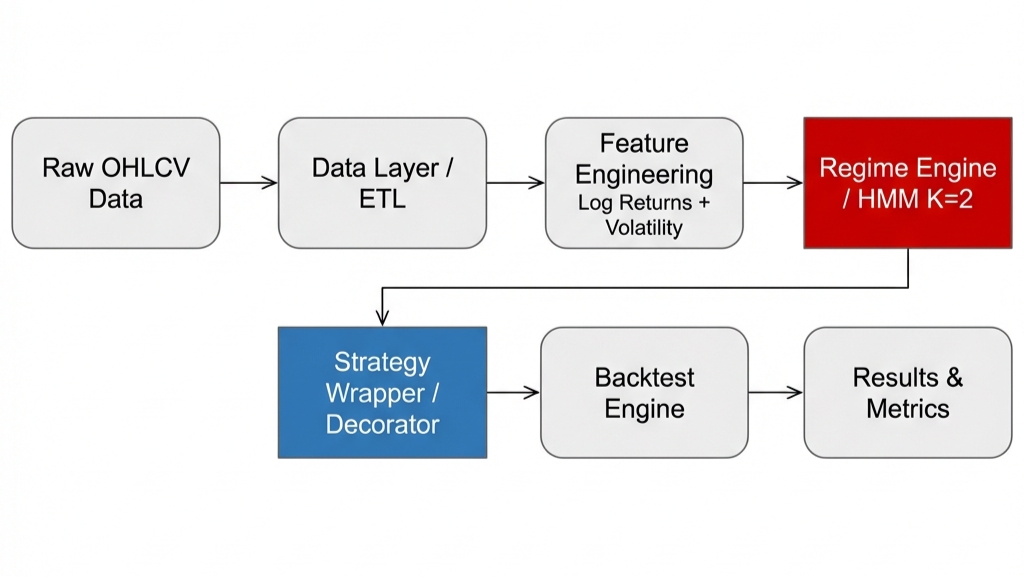
\includegraphics[width=0.55\columnwidth]{Fig_1.png}}
\caption{System Architecture Diagram. (This shows the different Implemented layers of the system)}
\label{fig:architecture}
\end{figure}

\subsection{The Data Layer}

As discussed in Fig.~\ref{fig:architecture}, The data layer is the ETL (Extract, Transform, Load) pipeline, it takes Raw OHLCV (Open, High, Close, Volume) Data from Yahoo Finance Python library, and computes Log Returns and Realized Volatility (21-day rolling standard Deviation). Then a clean Pandas Data Frame where every row has both price history and volatility features which are needed by regime detector. We used csv to ensure the experiments run on the exact same dataset further ensuring reproducibility.

\subsection{The Regime Engine}

We used Gaussian Hidden Markov Model (HMM), It implements a State sorting algorithm. Standard HMMs assign states randomly. This engine forces a specific state to always represent a specific volatility cluster only. It pre-calculates the Viterbi Path(likely sequence of hidden states) for the entire history to prevent prediction errors that are caused due to lack of states. \hl{This is computed in a retrospective manner and all trading decisions use a walk-forward procedure where only data up to time $t-1$ is used to infer the regime at time $t$."} 

\subsection{The Strategy Interface}

The strategy interface implements the User Provided (Base strategy) strategy and a strategy wrapper. This is an abstract class that forces all user strategies to implement a generate signal(row) method. This makes the system to be flexible with the strategy type. Doesn't matter if it is just moving average based or complex neural networks, the system will treat and evaluate them the same via the implementation of this interface. The Wrapper utilizes Decorator Design Pattern. Instead of modifying the user's code to add the regimes to it, we use the user's object inside a Wrapper that consists of Regime Aware functionality.

The System flow is as follows:
\begin{enumerate}
\item The Regime engine waits for a signal from the wrapper.
\item Wrapper confirms if we're in the safe regime.
\item If unsafe, the wrapper returns 0.
\item If safe, the wrapper then delegates the call to the user defined strategy and returns the calls from the base strategy.
\end{enumerate}

\subsection{The Backtest/Execution Engine}

This is just a Simulator. This engine creates 2 portfolio instances(base and Experimental), it proceeds evaluating the data step by step, providing the same market data row to both portfolio instances at the same time until the dataset is finished. This prevents ``look ahead bias'' and ``Synchronization Bias'' both strategies get the same price data while being entirely separate to create a fair testing environment.

\section{Experimental Methodology}

\subsection{Regime Detection}

The unobserved market regimes can be modelled using Gaussian Hidden Markov Model (HMM). Let the hidden regime at time $t$ be $S_t \in\{1,2,\ldots,K\}$ $O_t$. A Gaussian HMM is defined by:

Initial Regime Probabilities:
\begin{equation}
\pi_i = P(S_1 = i)
\end{equation}

State Transition Probabilities:
\begin{equation}
a_{ij} = P(S_t = j | S_{t-1} = i)
\end{equation}

Gaussian Emission For Observations:
\begin{equation}
P(O_t|S_t=k) \sim N(\mu_k, \sigma_k^2)
\end{equation}

So, the Full Model is:
\begin{equation}
P(O_1, \ldots, O_T, S_1, \ldots, S_T) = \pi_{S_1} \prod_{t=2}^{T} a_{S_{t-1}, S_t} \prod_{t=1}^{T} P(O_t | S_t)
\end{equation}

Where, $O_t$ = Observed Feature at time $t$, in this case $O_t = RV_t$, which the 21-day rolling volatility (Our Feature), $\mu_k$ is average volatility in regime $k$, and $\sigma_k^2$ refers to how spread-out volatility is in regime $k$.

\subsection{Feature Selection}

The markets can switch between calm and volatile conditions while we do not observe any large changes in the returns. Capturing volatility is not always successful when we use raw returns for it, so we use Realised Volatility, which is computed as 21 day rolling Standard Deviation of returns:
\begin{equation}
RV_t = \sqrt{\frac{1}{21} \sum_{i=t-20}^{t} (r_i - \bar{r})^2}
\end{equation}

where, $r_t$ refers to the daily returns, $\bar{r}$ would be the mean over the last 21 days. ``21'' is chosen as the trading month would consist of 21 sessions. This provides a smooth and reliable indication of regime shifts because volatility reacts faster than the prices in the moments of panic or stress.

Hence the Observed process in our HMM is:
\begin{equation}
O_t = RV_t
\end{equation}

\subsection{The Wrapper Architecture}

The wrapper is built upon the Decorator Pattern. It's a software design technique to wrap an existing component with an outer layer that adds extra rules or behaviour. The main purpose of this wrapper is to act as a gate on top of the internal trading logic rather than interfering with it. It checks the regime before allowing the Base Strategy to execute on the basis of its signals. Let $Signal_{Strategy}(t)$ be the Signal from the original user defined Strategy. Let $\mathbb{I}(\cdot)$ be an indicator function. If the model classifies the time $t$ as safe regime to trade, noted as $Regime_t = 0$, the signal will pass through otherwise it would be blocked.
\begin{equation}
Signal_{final}(t) = Signal_{Strategy}(t) \cdot \mathbb{I}(Regime_t = 0)
\end{equation}

This architecture cleanly separates the core trading logic away from the regime control system. This procedure in a lot of cases simply helps limit the risk, or even higher gains too. This makes the evaluation clean, one can clearly see if the regime adaptation adds to their edge and in what way, or even if that's the case or not with their strategy.

\subsection{Experimental Setup}

We tested this framework by taking daily SPY 500 data from 2000 to 2025, this time-period includes the ``Dot Com Crash'', the 2008, Global Financial Crisis, and the 2020 COVID Pandemic which cause Worldwide market shock. These types of events create volatility regimes that allow proper evaluation of regime identification. For testing purposes, we took a simple ``Mean Reversion strategy'' with a high-risk profile. The signal is:
\begin{equation}
RSI_t < 15 \rightarrow \text{Buy}
\end{equation}

This can perform really well in stable trending markets that are following an Elliot wave pattern but fails in fast drawdowns. Now due to this characteristic this is likely to blow the whole portfolio by the end of testing which is exactly what we will be testing by implementing the Regime-Aware system onto the strategy without touching or morphing any of its rules. We will observe how much risk can be limited on this testing portfolio just by making our failing strategy ``Regime-Aware''. To avoid look-ahead bias, model training and execution will follow a ``walk-forward'' process, The HMM will be fitting only onto the historical data up to time $t$, which refers to present in the back testing instance, this would be further used to predict regime at time $t+1$ and the window expand over time. This keeps the testing realistic without leaking future info which can skew the results of the model. \hl{The implementation uses $K = 2$ HMM states, 5 basis points transaction cost, and $10,000 USD$ initial capital, The code for which will be released upon publication.}

\section{Results and Analysis}

% ============================================
% FIGURE 2 PLACEHOLDER - Regime vs Base Strategy Equity Curve
% ============================================
\begin{figure}[htbp]
\centerline{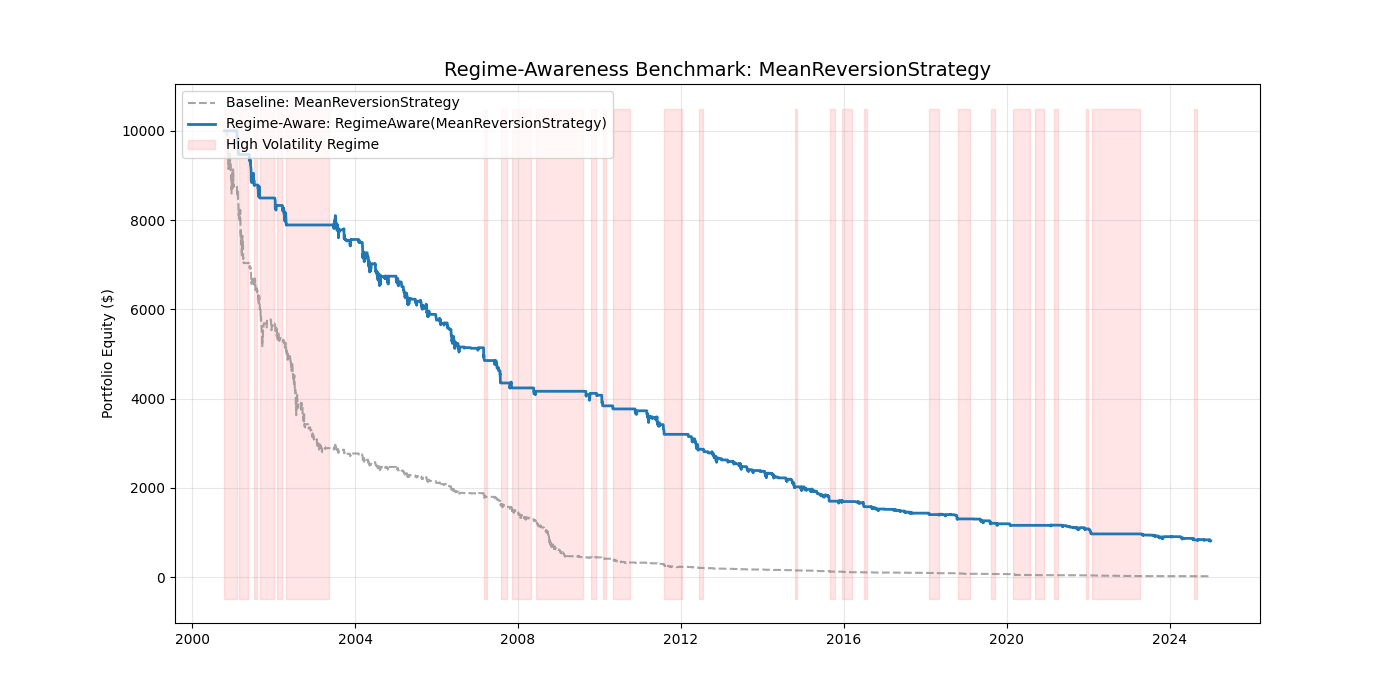
\includegraphics[width=\columnwidth]{benchmark_chart.png}}
\caption{\hl{Regime based vs Base Strategy. (Equity return graph)}}
\label{fig:equity}
\end{figure}

\subsection{Interpretation (as observed from Table~\ref{tab:results})}

\begin{enumerate}
\item[a)] Max Drawdown Improves from -99.8\% to -91.9\%.
\item[b)] Sharpe Ratio Improves, this indicates better risk efficiency.
\item[c)] Total Return still remains negative as the base strategy has no edge.
\end{enumerate}

As shown in the Fig.~\ref{fig:equity}, The same can be observed from the Equity time curve where the regime detection system properly detected major and few minor regimes of high stress as well. Also, the base strategy pretty much blew the whole account by 2008-2009, while the instance with Regime-Aware capabilities was able to survive till the end of 2025 with still around 800-900 USD in Portfolio. This proves that the improvement in risk limiting factor comes entirely from regime detection and protecting the strategy to make decisions during the time-periods of high stress and uncertainty, where the model is more likely to fail.

\begin{table}[htbp]
\caption{Strategy Evaluation}
\begin{center}
\footnotesize
\begin{tabular}{|p{2.2cm}|c|c|c|}
\hline
\textbf{Strategy} & \textbf{Total Ret.} & \textbf{Sharpe} & \textbf{Max DD} \\
\hline
Baseline Mean-Reversion & -99.81\% & -1.57 & -99.81\% \\
\hline
Regime-Aware & -91.88\% & -1.51 & -91.91\% \\
\hline
\end{tabular}
\label{tab:results}
\end{center}
\end{table}

\subsection{Why it worked}

Markets show a tendency of volatility clustering which essentially means, if the conditions are highly volatile, it tends to stay that way for a while, and similarly if the conditions are calm and non-volatile the same tendency would hold for these conditions as well. Due to this phenomenon volatility rises before major crashes. The HMM detects this shift into high volatility early enough to flag that as a regime change which in this case stops new trades. The Wrapper operating on this regime engine blocked the worst entries during the crisis which reduced the overall drawdown and collapse speed of our base strategy. The risk reduction was implemented without changing literally anything from our original trading logic.

\subsection{Maintaining the Integrity of the Specifications}

The cost can be the fact that this filter also activates during the small pullbacks which the regime engine might flag as regime change and hence filter out the possibly profitable trading opportunities. Due to regime filters the exposure to the market is limited to a great extent which leads to a lower return on a strategy that already has relatively no edge, this is something that is subject to evaluation by the user. The trade-off mentioned here is certainly intentional and needs to be analysed in order to find the optimal balance.

\subsection{Strategy Sensitivity}

The Testing strategy used here is mean reversion which benefits a lot because it fails during volatility spikes. This regime gating system's strength depends on the fact that in what ways the base strategy interacts with volatility.

\section{Conclusion}

The proposed framework here separates market regime analysis from trading logic. The wrapper architecture in this framework makes any existing strategy regime aware without rewriting the internal code or modifying it in any way. As a general risk filter, we implemented the Gaussian HMM which detects volatility shifts. Even weak strategy like mean reversion was observed with reduced risk factor and drawdown simply but introducing regime aware tendencies. The observed risk reduction was the resultant of regime gating which explains the framework's independent impact.  Also, it is modular so more advanced regime models can be added later with minimal change and the same applies to the user-based strategies, from simple statistical or technical models to complex neural network-based AI models. \hl{However its crucial to clarify that this framework is not to be interpreted as a universal performance enhancer rather contirbutes towards risk evaluation and mitigation. Moreover the final effectiveness of the system relies largely on the strategy itself with this framework only evaluating it effectiveness when the same if combined with risk-aware features.} Future work can include testing with more advanced profitable strategies, more advanced regime-based trading logic morphing to not only limit the losses but convert them into profitable positions.

\begin{thebibliography}{00}
\bibitem{b1} Hamilton, J. D. (1989). ``A New Approach to the Economic Analysis of Nonstationary Time Series and the Business Cycle.'' Econometrica 57(2).
\bibitem{b2} Rabiner, L. R. (1989). ``A Tutorial on Hidden Markov Models and Selected Applications in Speech Recognition.'' Proceedings of the IEEE 77(2), 257--286.
\bibitem{b3} Ang, A., \& Bekaert, G. (2002). ``International Asset Allocation with Regime Shifts.'' Review of Financial Studies 15(4), 1137--1187.
\bibitem{b4} Lo, A. W. (2004). ``The Adaptive Markets Hypothesis: Market Efficiency from an Evolutionary Perspective.'' Journal of Portfolio Management 30(5), 15--29.
\bibitem{b5} Nystrup, P., Madsen, H., \& Lindstr\"{o}m, E. (2015). ``Stylised facts of financial time series and hidden Markov models in continuous time.'' Quantitative Finance 15(9), 1531--1544.
\bibitem{b6} Castellano, R., \& Scaccia, L. (2007). ``Bayesian Inference for Hidden Markov Models and their Application to Financial Time Series.''
\bibitem{b7} Wu, P., \& Siwasarit, W. (2020). ``Capturing the Order Imbalance with Hidden Markov Model: A Case of SET50 and KOSPI50.'' Asia-Pacific Financial Markets 27(1), 115--144.
\bibitem{b8} Tsymbal, A. (2004). ``The Problem of Concept Drift: Definitions and Related Work.'' Technical Report TCD-CS-2004-15, Trinity College Dublin.
\bibitem{b9} Gama, J., \v{Z}liobait\.{e}, I., Bifet, A., Pechenizkiy, M., \& Bouchachia, A. (2014). ``A Survey on Concept Drift Adaptation.'' ACM Computing Surveys 46(4), 44.
\bibitem{b10} Cavalcante, R. C., Brasileiro, R. C., Souza, V. L. F., Nobrega, J. P., \& Oliveira, A. L. I. (2016). ``Computational Intelligence and Financial Markets: A Survey and Future Directions.'' Expert Systems with Applications 55, 194--211.
\bibitem{b11} Deldari, S., Smith, D. V., Xue, H., \& Salim, F. D. (2021). ``Time Series Change Point Detection with Self-Supervised Contrastive Predictive Coding (TS-CP$^2$).'' The Web Conference (WWW 2021).
\bibitem{b12} Nystrup, P., Madsen, H., \& Lindstr\"{o}m, E. (2016). Long Memory of Financial Time Series and Hidden Markov Models with Time-Varying Parameters. Journal of Forecasting, 36(8), 989--1002.
\bibitem{b13} Fons, E., Dawson, P., Yau, J., Zeng, X., \& Keane, J. (2021). ``A novel dynamic asset allocation system using Feature Saliency Hidden Markov Models for smart beta investing.'' Expert Systems with Applications 163, 113720.
\bibitem{b14} Wiese, M., Knobloch, R., Korn, R., \& Kretschmer, P. (2020). ``Quant GANs: Deep Generation of Financial Time Series.'' Quantitative Finance 20(9), 1419--1440.
\bibitem{b15} Karassavidis, I. et al. (2025, working paper). ``Quantitative Evaluation of Volatility-Adaptive Trend-Following Models in Cryptocurrency Markets (November 28, 2025).'' SSRN preprint.
\bibitem{b16} Backtrader Project (2015--2024). Backtrader: A Feature-Rich Python Framework for Backtesting and Trading. Documentation and source at backtrader.com and GitHub.
\bibitem{b17} Quantopian, Inc. (2013--2024). Zipline: A Pythonic Algorithmic Trading Library. GitHub project and documentation, event-driven backtesting engine.
\bibitem{b18} QuantConnect (2015--2024). LEAN Algorithmic Trading Engine. Open-source, multi-asset backtesting and live trading engine powering QuantConnect.

\end{thebibliography}

\end{document}
